\documentclass[a4paper,conference]{IEEEtran}
\usepackage{cite}
\usepackage[dvipdfmx]{graphicx}
\usepackage{booktabs}
\usepackage{amsthm, amsmath, amssymb, amsfonts} % math mode
\usepackage{bm} % bold
\usepackage{comment}
\usepackage{latexsym}

\usepackage{url}

% correct bad hyphenation here
\hyphenation{op-tical net-works semi-conduc-tor}

\begin{document}
% Do not put math or special symbols in the title.
\title{Tsallis Entropy Based Labelling}

\author{\IEEEauthorblockN{Kentaro Goto}
\IEEEauthorblockA{Waseda Univ., JP\\
Email: kentaro.goto@asagi.waseda.jp}
\and
\IEEEauthorblockN{Masato Uchida}
\IEEEauthorblockA{Waseda Univ., JP\\
Email: m.uchida@waseda.jp}
}

\maketitle

% As a general rule, do not put math, special symbols or citations
% in the abstract
\begin{abstract}
The abstract goes here.
\end{abstract}

% no keywords

\IEEEpeerreviewmaketitle

\section{Introduction}
%教師あり分類学習における「インスタンスに対する正確なラベル付け問題」の重要さとその困難さ(←コストとはいわない)
インスタンスに付与されるラベルの正確さを確保することは,教師あり分類学習における重要な要件の一つである.
これは,教師あり分類学習により獲得される分類モデルの精度が,インスタンスに付与されるラベルの正確さに強く依存するためである.
しかし,インスタンスが所属するクラスがアノテータにとって明らかでない場合,そのインスタンスに付与すべきラベルを正確に選択することは困難である.
Ishida等は,この困難さを軽減するために,インスタンスが「所属する」クラスを表すラベル(ordinary label)ではなく,「所属しない」クラスを表すラベル(complementary label)を付与する場合における教師あり分類学習を定式化した.
与えられたインスタンスが所属するクラスがアノテータにとって明らかではない場合,そのクラスを特定してordinary labelを付与するよりも,complementary labelを付与する方が容易であると考えることは自然である.

%単一のcomplementary label/ordinary labelの概念を一般化したcandidate labelの紹介
インスタンスに対して単一のcomplementary labelを付与することは,それ以外のすべてのラベルをordinary labelの候補にすることと等価である.
Katsura等は,ordinary labelの候補となるラベルをcandidate labelと呼んだ.
インスタンスに対して単一のordinary labelを付与することは,candidate labelの個数が1つであることに対応する.
彼らは,この観点から,単一のordinary/complementary labelがインスタンスに付与された場合の学習を一般化し,複数のcandidate labelsがインスタンスに付与された場合における学習を定式化した.

%candidate labelsの個数が予め固定されることの弊害の指摘
Ishida等,Katsura等の定式化においては,インスタンスに対して付与されるcandidate labelsの個数はすべてのインスタンスに対して共通である.
すなわち,これらの定式化においては,「予め指定された同数のラベルをすべてのインスタンスに対して一律に付与しなくてはならない」という制約をアノテータに課すということを暗黙に仮定している.
しかし,この制約は,アノテータの能力に相応したラベル付けを困難なものとし,教師あり分類学習における重要な要件であるラベル付けの正確さの成立を妨げる.
例えば,与えられたインスタンスが所属するクラスがアノテータにとって明らかであるにもかかわらず単一のcomplementary labelを付与しなければならない場合,その制約がアノテータにとっての妨げとなり,正確なラベル付けが期待できない.

%本論文の核心となるアイデア(確信度に応じたラベル付けという考え方)の提示
この問題の原因は,ラベル付けの対象となるインスタンスが所属するクラスについてアノテータが考える不確からしさ,uncertainty(あるいは確からしさ,certainty)はすべてのインスタンスについて均一であるとは限らず,それぞれのインスタンスについてまちまちであることにある.
インスタンスが所属するクラスとして不確からしさが低い場合(確からしさが高い場合)には該当するラベルをすべて付与し,そうではない場合にはラベルを付与しない,というように,アノテータの判断によりそれぞれのインスタンスに対してラベル付けするならば,付与するラベルの個数に関する不自然な制約が加えられることはなく,正確なラベル付けを期待できる.
本論文では,この着想に基づき,「インスタンスが所属するクラスについてアノテータが考える不確からしさ(確からしさ)が,ある閾値を下回った(上回った)場合に,それに該当するすべてのクラスのラベルを付与する」という原理に基づくラベル付けの振る舞いについて検討し,その特徴を明らかにする.

%数理構造の美しさを強調する
本論文では,この不確からしさ(確からしさ)をTsallis self information,閾値をTsallis endtorpyにより定量的に表現する枠組み,Tsallis entropy based labelling,を提唱する.
Tsallis entropyは,Shannon entropyを非加法的に拡張したものである.
Tsallis entropyの非加法性はパラメータ$q>0$により制御され,$q\rightarrow 1$の場合がShannon entropyに相当する.
Tsallis entropy based labellingは,インスタンスのラベル付けにおける二つの標準的な手法を特別の場合として含んでいる.
一つ目は,インスタンスが所属するクラスについての確率が最も大きいものに対応するラベルを付与するという方法である.
この方法は,インスタンスに対して単一のordinary labelを付与する上で自然である.
本論文では,この方法が,Tsallis entropy based labellingにおいては,$q\rightarrow\infty$の場合に相当することを示す.
二つ目は,インスタンスが所属するクラスについての確率が$1/K$を超えるものに対応するすべてのラベルを付与するという方法である.
ここに,$K$は総クラス数を表す.
この方法は,インスタンスに対して複数のordinary labelを付与する上で自然である.
本論文では,この方法が,Tsallis entropy based labellingにおいては,$q\rightarrow 0$の場合に相当することを示す.
以上の結果は,Tsallis entropy based labellingが,インスタンスのラベル付けにおける諸手法を一般化したものであることを意味している.

%冒頭の前振りで示したラベル付けの正確さという課題(建前上の目標規定文(より強調したいのは↑の数理構造の美しさ))が解消されたことを示す
また,本論文では,Tsallis entropy based labellingにより付与されたラベルの正確さを,予め指定された同数のラベルをすべてのインスタンスに対して一律に付与する手法における正確さと比較する.
具体的には,インスタンスが所属するクラスについての確率の上位$r$個($r \in \mathfrak{R}$)に対応するラベルを付与する手法(top-$r$)との比較を行う.
数値実験によって,Tsallis entropy based labellingにより付与されたラベルの正確さは,top-$r$により付与されたラベルの正確さよりも高いということを示す.
このことは,インスタンスに付与するラベルの個数を同数に固定するという制約を課さずに,アノテータが感じる不確かさに応じて自由に選択させることで,インスタンスに付与されるラベルの正確さが向上することを示唆する.

%お約束の論文の構成について
本論文の構成は以下の通りである.
第2節では,,,

\section{Related Work}
教師あり分類学習の全体プロセスの出発点は,与えられたインスタンスに対してラベル付けするためのアノテーションを行うことである.
これにより,学習の実行に必要となる訓練データを準備することができる.
本節では,アノテーションに関する既存手法を概観し,本研究の位置付けを明確にする.
\ref{subsec:cost_reduction}節では,大量のインスタンスに対するラベル付けの作業を効率化するための既存手法について紹介する.
\ref{related_comp-labels}節では,インスタンスとそれに対応するラベルの関係が一対一とは限らない場合における機械学習の概念について紹介する.
また,そのようなラベル付けを行うアノテータの振る舞いを規定するモデルについても紹介する.

%しかし,教師あり機械学習の全体プロセスの中で中心課題とされるのは,インスタンスは予め準備されたものとし,それを用いた学習方法を改善することであることが多く,インスタンスに付与されるラベルの質の向上に関する議論は多くない.
%本研究では,entropy labellingという新たな枠組みの定式化と評価を通じ,インスタンスに対する高品質なラベル付けを行うための方法論について検討する.
%このような検討は,著者らの知る限り,これまでに行われていない.

\subsection{アノテーションの効率化に関する研究}\label{subsec:cost_reduction}
静止画,動画,3Dモーション,自然言語,ゲノム情報といった様々な応用領域におけるアノテーションの研究が活発に行われている\cite{Zhang:2012,Russakovsky:2015,Muller:2009,Bird:2013,Richardson:2012}.
こうした応用領域におけるアノテーションにおいては,高度な専門性に基づいた人間の解釈が求められることがあり, ルールベースの単純な自動アノテーションでは,その精度を確保することが難しい場合がある.
一方で,人間による手動アノテーションは一般に高コストなため,アノテーションの手続きの工夫による効率化が必要である.
そのため,このような具体的な応用領域におけるアノテーションについては,それぞれの応用領域に特有の条件を加味することで,精度と効率を両立するための手法が検討されている.

また,active learningを用いることで,アノテーションを効率化する手法が提案されている.
Active learningは,ラベルが付与されていないインスタンスの中から,分類モデルの性能向上に有効であると期待されるものから順にラベルを付与して学習する手法である.
ラベルを付与すべきインスタンスを選択する手法は,訓練モデルの性能向上に寄与すると期待される度合いを評価する方法や,適用する機械学習アルゴリズムの違いにより数多く提案されている \cite{Settles:2009,Wang:2011}.
%例えば,Beaugnon等により提案された異常検知システムでは,悪性/良性というラベルに加え,データをクラスタリングした際のクラス情報を利用してラベル付けするデータを選択する手法を採用している \cite{Beaugnon:2017}.
例えば,Schein等は,ロジスティック回帰にactive learningを適用する手法を提案している\cite{Schein:2007}.
また,Fukushi等は,識別境界に近いデータに対してラベルを付けるというactive Learningをensemble learningと組み合わせる手法を提案し,それを悪性ドメイン名の検知に応用した \cite{Fukushi:2019}.

\subsection{多様なラベル付きデータを用いた学習に関する研究}\label{related_comp-labels} 
インスタンスに付与されるラベルには,その形式の違いによって,いくつかに分類される.
図~\ref{fig:rw}に代表的なラベル付けの種類を示す.
最も素朴なものは,(a)のordinary labelであり,一つのインスタンスに対し,一つのラベルが付与される.
また,(b)no supervisionにおいては,インスタンスはラベルを持たない.
(a)と(b)を混合した枠組みを(c)semi-supervisionという.
さらに,一つのインスタンスに対してラベルの集合が付与されるものを(d)multi-labelsといい,インスタンスの集合に対して一つのラベルが付与されるものを(e)multi-instancesという.ただしmulti-labelsにおける複数のラベルは,すべてインスタンスがもつ複数の性質を表す正しいラベルである~\cite{Tsoumakas:2009}.一方でmulti-instancesにおいては,インスタンスの集合とラベル一つが対となっており,実際にはそのうち最大で一つのインスタンスのみがラベルと紐づく~\cite{Dietterich:1997}.

\begin{figure*}[t]
\begin{center}
    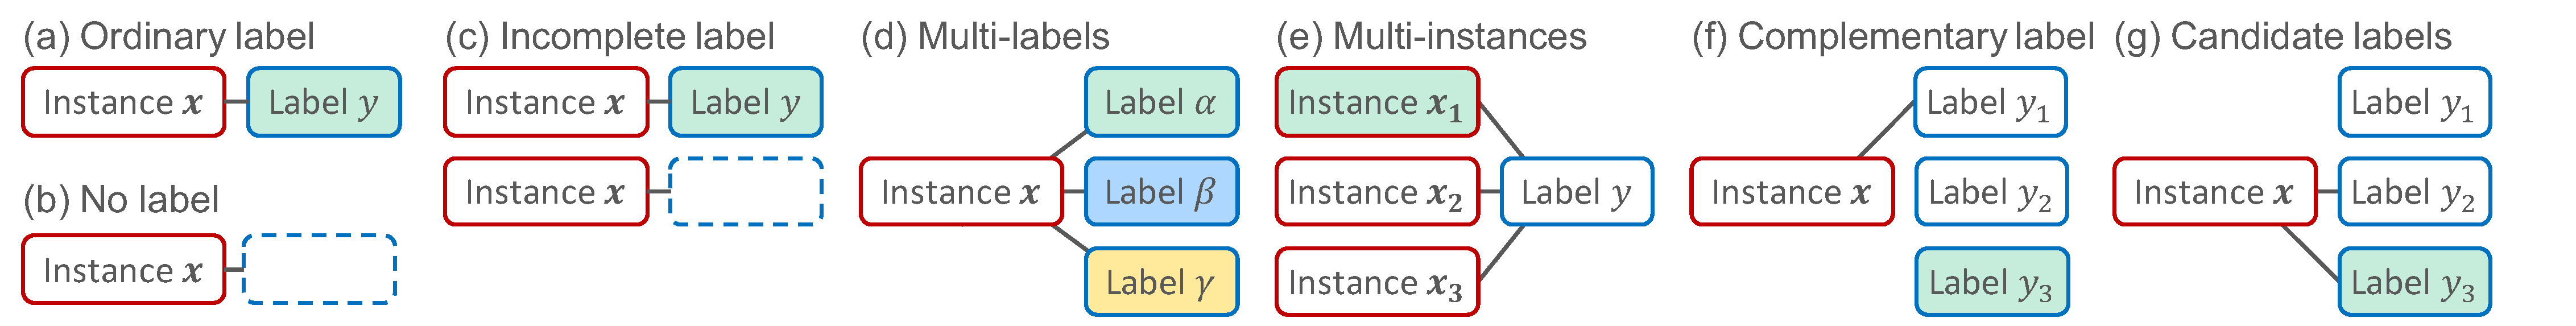
\includegraphics[width=1.0\textwidth]{figs/graphs/rw_labels.pdf}
    \caption{機械学習における様々なラベル付けの種類}
    \label{fig:rw}
\end{center}
\end{figure*}

Ishida等は,インスタンスが所属するクラスがアノテータにとって明らかでない場合に対応するために,インスタンスが所属しないクラスをラベルとするアノテーションを提案している \cite{Ishida:2017}.
このようなラベルはcomplementary labelと呼ばれる(図~\ref{fig:rw}中の(f)).
Ishida等は,complementary labelが付与されたインスタンスを生成する確率分布を,それがordinary labelではない確率によって定義した.
また,Ishida等の結果の一般化に関する研究が行われている.
Katsura等は,インスタンスに対してcomplementary labelsを付与することは,それ以外のすべてのラベルをordinary labelの候補にすることと等価であるということに着目し,ordinary labelの候補となるcandidate labels(図~\ref{fig:rw}中の(g))が付与されたインスタンスを生成する確率分布を定義した \cite{Katsura:2020}.
これと等価な確率分布はCao等によっても独立に定義されている \cite{Cao:2020}.
また,Feng等は,任意個数のラベルが付与されたインスタンスを生成する確率分布を定義している \cite{Feng:2019}.
これらの一連の研究により定義された確率分布は,アノテータによるラベル付けの振る舞いを表現するモデルであると捉えることができる.
しかし,これらの確率モデルにおいては,アノテータが感じる不確かさが与えるインスタンスの精度への影響については議論されていない.
本研究では,「インスタンスが所属するクラスについてアノテータが考える不確からしさ(確からしさ)が,ある閾値を下回った(上回った)場合に,そのクラスのラベルを付与する」という原理に基づくラベル付けの振る舞いについて検討し,その特徴を明らかにする.

\section{Formulation of Tsallis Entropy Based Labelling}
\subsection{Tsallis Entropy}
有限集合$\mathcal{S}$上に定義された至るところ正の確率分布$p$を$p(s) > 0$, $\sum_{s\in\mathcal{S}}p(s)=1$と定義する.
このとき,$q \in \mathfrak{R}$について,確率分布$p$のTsallis entropy $H_{q}(p)$は以下のように定義される \cite{Tsallis:1988}.
\begin{align}
    H_{q}(p) = \frac{1}{q-1}\left(1-\sum_{s \in \mathcal{S}}p(s)^{q}\right)\label{eq:tsallis-entropy}
\end{align}
式\eqref{eq:tsallis-entropy}において$q \rightarrow 1$とすると,Shannon entropy $H(p)$が得られる.
すなわち,
\begin{align}
    \lim_{q \rightarrow 1}H_{q}(p) = - \sum_{s \in \mathcal{S}} p(s) \ln p(s) \equiv H(p)\label{eq:shannon-entropy}
\end{align}
となる.

式\eqref{eq:tsallis-entropy}は,以下のように書き換えることができる.
\begin{align}
    H_{q}(p)
    &= \sum_{s \in \mathcal{S}}p(s)\left\{\frac{1}{q-1}(1-p(s)^{q-1})\right\}\nonumber\\
    &=\mathbb{E}_{p}\left[\frac{1}{q-1}\left(1 - p(s)^{q-1}\right)\right]\nonumber\\
    &= \mathbb{E}_{p}[h_{q}(p(s))]
\end{align}
ここで,$\mathbb{E}_{p}$は$p$に関する期待値を表す.
また,$h_{q}(p(s))$はTsallis self-informationと呼ばれ,以下のように定義される.
\begin{align}
    h_{q}(p(s)) = \frac{1}{q-1}\left(1 - p(s)^{q-1}\right)\label{eq:tsallis-self-information}
\end{align}
式\eqref{eq:tsallis-self-information}において$q \rightarrow 1$とすると,Shannon self-information $h(p(s))$が得られる.
すなわち,
\begin{align}
    \lim_{q \rightarrow 1}h_{q}(p(s)) = - \ln p(s) \equiv h(p(s))\label{eq:shannon-self-information}
\end{align}
となる.

\subsection{Definition}
教師あり分類学習においては,入力$x$と,それが所属するクラスを表すラベル$y \in \mathcal{Y}$を対にした訓練データが必要となる.
$K~(\geq2)$値分類問題においては,$|\mathcal{Y}| = K$となる.
インスタンス$x$が与えられたとき,それが所属するクラスが$y$となる条件付き確率を$p_{x}(y)$と表す.
この条件付き確率分布は,機械学習の文脈においては,真の分布と呼ばれる.
アノテータによるラベル付けにより訓練データを生成する場合においては,入力$x$が与えられたとき,それが所属するクラスが$y$であるとアノテータが考える条件付き確率が$p_{x}(y)$に対応する.
通常,条件付き確率$p_{x}(y)$に従って選択された一つのラベルが入力$x$に対して付与されることが暗黙に仮定されている.

インスタンス$x$が所属するクラスについてアノテータが考える不確からしさがこの条件付き確率$p_{x}(y)$により定まるものとし,それを$f(p_{x}(y))$と表す.
本論文では,この不確からしさ$f(p_{x}(y))$が,ある閾値を下回った場合にそのクラスのラベルを付与する,という原理に基づくラベル付けの振る舞いについて調べる.
また,この閾値は,条件付き確率分布$p_{x}$の汎関数$\theta(p_{x})$として定まるものとする.
具体的には,この閾値$\theta(p_{x})$を,$f(p_{x}(y))$の$p_{x}(y)$に関する期待値として以下のように定義する.
\begin{align}
    \theta(p_{x})
    = \mathbb{E}_{p_{x}}[f(p_{x}(y))]
    = \sum_{y \in \mathcal{Y}}p_{x}(y)f(p_{x}(y))
\end{align}
すなわち,この原理においては,入力$x$に対し,$f(p_{x}(y)) \le \theta(p_{x})$を満たすすべての$y \in \mathcal{Y}$がラベルとして付与される.
閾値$\theta(p_{x})$は可変であることから,付与されるラベルの個数も可変である.

ここで,$f(\cdot)=h_{q}(\cdot)$とすると,不確からしさ$f(p_{x}(y))$は$p_{x}(y)$に関するTsallis self-informationに対応し,閾値$\theta(p_{x})$はTallis entropyに対応する.
このラベル付けの方法を,本論文では,Tsallis entropy based labellingと呼ぶ.

\subsection{Examples}\label{subsec:example_models}

Tsallis entropy based labellingには,典型的に考えられるいくつかのラベル付け手法が特別な場合として含まれている.
以下では,それらについて説明する.

\subsubsection{$q \rightarrow 0$の場合}
式\eqref{eq:tsallis-entropy}, \eqref{eq:tsallis-self-information}より,
\begin{align}
    f(p_{x}(y)) &= \frac{1-p_{x}(y)}{p_{x}(y)}\label{eq:uncertainty-q=0}\\
    \theta(p_{x}) &= K -1\label{eq:threshold-q=0}
\end{align}
となる.
式\eqref{eq:uncertainty-q=0}より,$x$の所属するクラスが$y$であることについての不確からしさ$f(p_{x}(y))$が,$x$の所属するクラスが$y$である確率$p_{x}(y)$と,そうではない確率$1-p_{x}(y)$の比によって定められることがわかる.
また,\eqref{eq:threshold-q=0}は,閾値がクラスの総数に依存することがわかる.
このとき,
\begin{align}
    f(p_{x}(y)) \le \theta(p_{x}) \Leftrightarrow p_{x}(y) \ge \frac{1}{K}\label{eq:rule-q=0}
\end{align}
が成り立つ.
式\eqref{eq:rule-q=0}より,Tsallis entropy based labellingには,$x$の所属するクラスが$y$である確率$p_{x}(y)$が,$x$の所属するクラスを無作為に選ぶ場合の確率よりも大きい場合にラベル$y$を付与する,という手法が特別な場合として含まれることがわかる.
本論文においては,この手法を$1/K$ labellingと呼ぶ.

\subsubsection{$q \rightarrow 1$の場合}
式\eqref{eq:tsallis-entropy}, \eqref{eq:tsallis-self-information}より,
\begin{align}
    f(p_{x}(y)) &= h(p_{x}(y)) = - \ln p_{x}(y)\label{eq:uncertainty-q=1}\\
    \theta(p_{x}) &= H(p_{x}) = - \sum_{y \in \mathcal{Y}} p_{x}(y) \ln p_{x}(y)\label{eq:threshold-q=1}
\end{align}
となる.
式\eqref{eq:uncertainty-q=0}より,$x$の所属するクラスが$y$であることについての不確からしさ$f(p_{x}(y))$が,$x$の所属するクラスが$y$である確率$p_{x}(y)$のShannon self-informationによって定められることがわかる.
また,\eqref{eq:threshold-q=0}は,閾値が$p_{x}(\cdot)$のShanonn entropyによって定められることがわかる.
このとき,
\begin{align}
    f(p_{x}(y)) \le \theta(p_{x}) \Leftrightarrow p_{x}(y) \ge \exp(-H(p_{x}))\label{eq:rule-q=1}
\end{align}
が成り立つ.
一般に,$H(p_{x}) \le \ln K$であることから,$\exp(-H(p_{x})) \ge 1/K$となる.
したがって,式\eqref{eq:rule-q=1}の手法により入力$x$に付与されるラベルの個数は,式\eqref{eq:rule-q=0}の手法よりも少なくなる.
本論文においては,この手法をShanonn entropy-based labellingと呼ぶ.

\subsubsection{$q \rightarrow \infty$の場合}
以下が成り立つ.
\begin{align}
    &\lim_{q \rightarrow \infty} \frac{\frac{1}{q-1}-H_{q}(p_{x})}{\frac{1}{q-1}-h_{q}(p_{x}(y))}\nonumber\\
    &=\lim_{q \rightarrow \infty} \sum_{z \in \matycal{Y}} p_{x}(z) \left(\frac{p_{x}(z)}{p_{x}(y)}\right)^{q-1}\nonumber\\
    &
    \begin{cases}
    \le 1, & \text{if~}p_{x}(y) = \max_{z\in\mathcal{Y}}p_{x}(z)\\
    = \infty, & \text{otherwise}
    \end{cases}
\end{align}
%よって,$q \rightarrow \infty$のとき,
%\begin{align}
%    h_{q}(p_{x}(y)) \le H_{q}(p_{x}) ~\text{iff}~ p_{x}(y) = \max_{z \in \mathcal{Y}}p_{x}(z)
%\end{align}
%となる.
よって,
\begin{align}
    f(p_{x}(y)) \le \theta(p_{x}) \Leftrightarrow p_{x}(y) = \max_{z \in \mathcal{Y}}p_{x}(z)\label{eq:rule-q=infty}
\end{align}
が成り立つ.
式\eqref{eq:rule-q=infty}より,Tsallis entropy based labellingには,$x$の所属するクラスが$y$である確率が最も大きいときに,それに対応するラベルを付与する,という手法が特別な場合として含まれることがわかる.
本論文においては,この手法をtop-$1$ labellingと呼ぶ.

\section{Experimental settings}\label{sec:experimental_settings}
本節では、Tsallis entropy based labellingを用いたラベル付けの正確さを評価するために数値実験を行う。
本実験は,アノテータにラベルづけをさせるプロセス,そして得られたラベルの正確さを評価する指標を計算するプロセスの2つで構成される.
%まず使用するデータセットに対するアノテータの挙動を事前調査し,その結果を元に実験を行う.
以下では,事前調査と実験に共通する処理と,使用したデータセットについて述べる.

\subsection{アノテータによるラベルづけ}\label{subsec:annotation_process}
Tsallis entropy based labellingは、インスタンス$x$が与えられたとき、それが所属するクラスが$y$であるとアノテータが考える条件付き確率分布$p_{x}(\cdot)$を用いて定義される.

節では、この条件付確率分布$p_{x}(\cdot)$



本節では,本論文の実験における基礎となる,アノテータによるラベルづけについて述べる.はじめに訓練データを一定数用意し,従来通りに学習器に与えて学習させる.ここで得られる学習器を,本論文ではアノテータと呼ぶ.続いて,アノテータに対して,訓練データと重複のないインスタンスの集合を一定数与える.アノテータは,与えられたインスタンスに対して,その時々で与えられる異なった作業方針にしたがってラベルを付与する.具体的にラベルを付与する際の基準は,前述の通りその時々によって変化する.ラベルを付与する対象のインスタンスを学習器に与え,そのインスタンスが各クラスに属する確率を学習器に計算させた値を基に採用すべきラベルを決定するという構造は共通とする.アノテータによって生成された各インスタンスに対するラベルは,パラメータとして与えられる「方針」に沿ったものであり,その中でも従来通りの単一のラベルである場合と,複数のラベルである場合がある(ranges from 1 to K - 1 for K classes problems).

\subsection{生成されたラベルの評価}\label{subsec:labels_evaluation}
本節では,アノテータによって生成されたラベルの評価指標; ラベルの精度と平均ラベル数の計算について述べる.ラベルの精度を計算するには,まずラベルをインスタンスごとに分解し,元のデータセットにおける正解ラベルと一致する数をカウントする.続いて,アノテータが正解したラベルの数を,生成されたラベル全体の総数で割ることで得られる数値をラベルの精度と定義する.
% [↑ここは図が必要?] %
一方で平均ラベル数は,生成されたラベルの総数を,ラベルを付与する対象としてアノテータに与えたインスタンス数で割ったものと定義する.以上の2つの指標; ラベルの精度と平均ラベル数を用いて,アノテーション作業方針間での違いを評価する.

\subsection{実装}\label{subsec:implementation}
本研究における実験の実装は全てPythonで行い,機械学習のライブラリにはscikit-learnを使用した.なお,~\ref{subsec:annotation_process}節で述べた学習器作成の際には,本研究においては本質的ではないため,特別な特徴量設計やハイパーパラメータの調整は行っていない.学習のモデルには多クラス分類のLogistic Regressionを選択した.

\subsection{データセット}\label{subsec:dataset}
本実験では,手書き数字の画像データセットであるMNISTを使用する.MNISTには訓練データとして$50000$件,テストデータとして$10000$件が用意されている.~\ref{subsec:annotation_process}節で触れたアノテータを作成する際の学習には,用意された訓練データのうち,計$2000$件を訓練データとして与え,精度(accuracy)は$10$クラス問題の場合で$83.04\%$で固定した.一方で,アノテータに新たにラベルを付与させるデータも各$K$クラス問題に対して計$2000$件で固定した.

\subsection{事前調査}\label{subsec:preliminary_exp}
実験の前に,MNISTに対するTsallis entropy based labellingとtop-$k$ labellingの挙動を確認する.MNISTは$10$クラス問題だが,クラス数による変化を観察するため,$2$クラス問題から$9$クラス問題までの全クラスの組合せ,および$10$クラス問題におけるアノテーションを扱う.すなわち,$K$クラス問題においては,$\binom{10}{K}$通りのクラスの組合せがあり,それら全てでアノテーション実験を行って得られるラベル精度と平均ラベル数の平均をとったものを最終的な$K$クラス問題における結果とする.Tsallis labellingでは,$q\in[0, 0.1, 0.5, 1.0, 2.0, 10.0, \infty]$で変動させる.ただし,$q = 0$と$q = 1.0$と$q = \infty$の場合はいずれも極限値であり,そのまま$q$の値として代入して計算することは不可能である(undefinedになる)ため,それぞれ理論的に等価(第\ref{subsec:example_models}節参照)な$1/K$ labelling($K$は総クラス数),Shannon labelling,top-$1$で代用する.
一方,top-$k$ labellingでは$k\in[1, 2, ..., 9]$で変動させる.ただし$k$を与える際には,$K$クラス問題に対してはtop-$(K
- 1)$以下を設定しなければならない.

以上を踏まえて,$q$を変化させたときのTsallis entropy based labellingと,$k$を変化させたときのtop-$k$ labellingによるアノテーションを実験で再現し,それぞれに対するラベル精度と平均ラベル数を計算した.まずTsallis entropy based labellingについて,図~\ref{fig:tsallis_acc}にクラス数とラベル精度の関係を表したグラフを示す.なお,横軸がクラス数を,縦軸がラベル精度を表す.さらに,図~\ref{fig:tsallis_ave_lnum}にはクラス数と平均ラベル数の関係を表したグラフを示す.こちらでは横軸がクラス数を,縦軸が平均ラベル数を表す.

% Tsallis entropy based labellingにおけるラベル精度-クラス数の関係
\begin{figure}[t]
\begin{center}
    % ファイル名に"_"が入っていると数式モードと認識されるようなので,とりあえず"-"で置き換えています %
    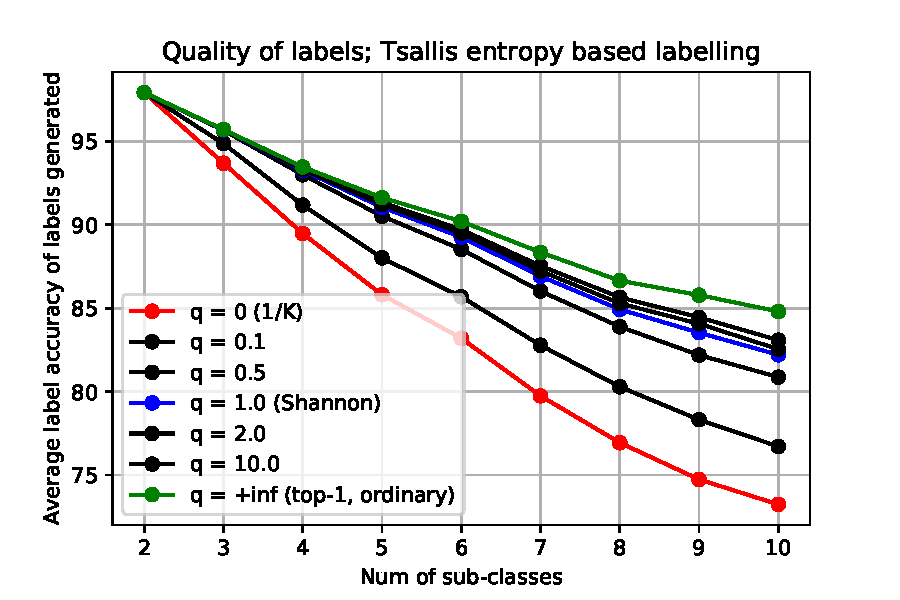
\includegraphics[width=1.0\linewidth]{figs/graphs/tsallis-qs.pdf}
    \caption{Tsallis entropy based labelling - accuracy curve}
    \label{fig:tsallis_acc}
\end{center}
\end{figure}

% Tsallis entropy based labellingにおけるクラス数-平均ラベル数の関係
\begin{figure}[t]
\begin{center}
    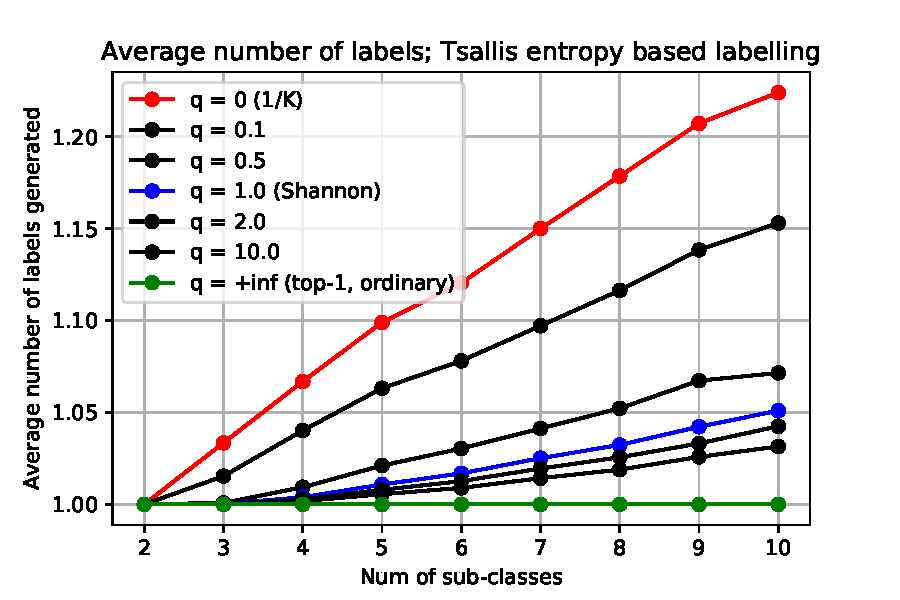
\includegraphics[width=1.0\linewidth]{figs/graphs/tsallis-qs-lnum.pdf}
    \caption{Tsallis entropy based labelling - average number of labels per data}
    \label{fig:tsallis_ave_lnum}
\end{center}
\end{figure}

図~\ref{fig:tsallis_acc}を参照すると,パラメータ$q$を大きくするほどラベル精度が向上する様子が現れている.一方で図~\ref{fig:tsallis_ave_lnum}を参照すると,$q$を大きくするほど平均ラベル数は減少し,$1.00$に近づいていく.以上の2つから,パラメータ$q$は,いかに少数のcandidate labelsにまで絞り込むか,すなわちアノテータの積極度を表した指標であることが実験的に示された.

% ここは自然なことなので蛇足?
\begin{comment}
また,図~\ref{fig:tsallis_acc},図~\ref{fig:tsallis_ave_lnum}共に,クラス数の増加によってラベルの質が低下することを示している.すなわち,クラス数が増加すると図~\ref{fig:tsallis_acc}ではラベルの精度が低下し,図~\ref{fig:tsallis_ave_lnum}では平均ラベル数が増加する様子がみてとれる.これは,クラス数の増加が問題の複雑化に貢献することが由来であり,どちらも自然な結果である.
\end{comment}

次に,図~\ref{fig:top-k}にクラス数とtop-$k$ labellingのラベル精度の関係を示す.
% top-$k$ labellingのラベル精度-クラス数の関係
\begin{figure}[t]
\begin{center}
    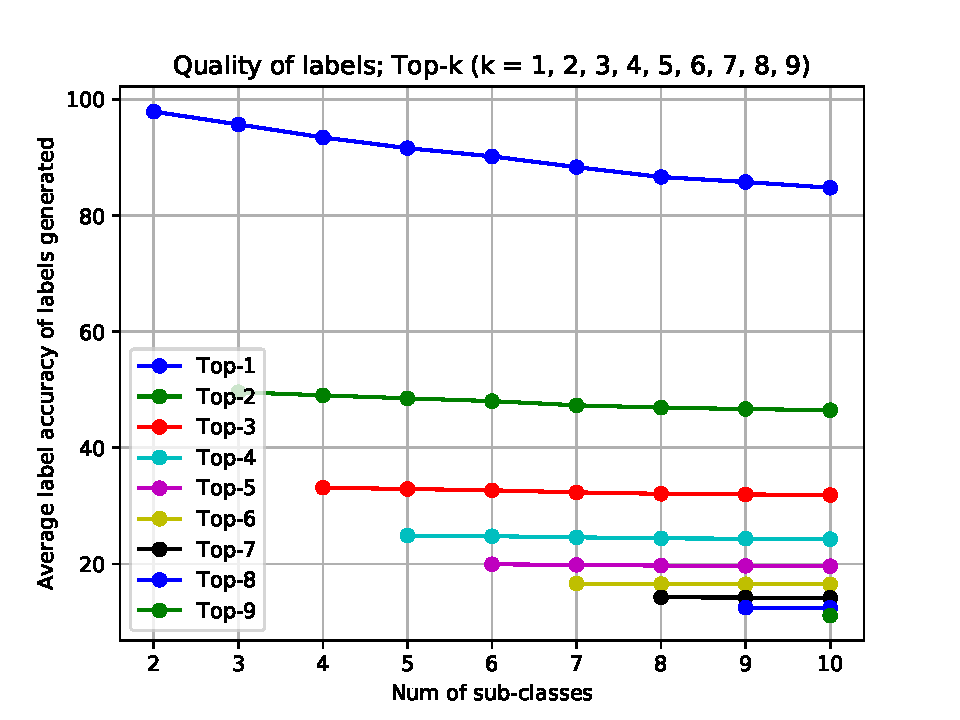
\includegraphics[width=1.0\linewidth]{figs/graphs/topk-labels-acc.pdf}
    \caption{top-$k$ labelling - accuracy curve}
    \label{fig:top-k}
\end{center}
\end{figure}

top-$k$では,クラス数の増加に伴って緩やかに精度は低下するものの,Tsallis entropy based labellingほどの変化はない.一方で,$k$の変化に対する精度の変化は,top-$1$以降は急激に低下することがわかる.ただしtop-$k$においては平均ラベル数は$k$で固定されるため,これら2つの特徴で単純にTsallis entropy based labellingとの比較に用いることはできない.そこで,以上の結果を基に平均ラベル数とラベルの精度の組合せで比較実験を行う.

\subsection{実験}\label{subsec:experiment}
%.書き直し top-rという名前は使わない 
Tsallis entropy based labellingでは平均ラベル数は実数値をとるが,top-$k$の場合には$k \in \mathfrak{N}$で固定になるため,2つのアノテーション手法間の単純な比較はできない.そこで本実験では,Tsallis entropy based labellingによるアノテーションと,
異なる2つの$k$の値についてのtop-$k$を組み合わせたアノテーションを,ラベルの精度と平均ラベル数の観点から比較する.
異なる$k$についてtop-$k$を組み合わせ,得られたラベルをひとまとまりに扱う場合,その平均ラベル数は実数となる.したがって,top-$k$の平均ラベル数を擬似的に実数に拡張することができ,Tsallis entropy based labellingとの直接の比較が可能となる.
$k$の値の組合せ方は様々あるが,今回は実装上top-$1$とtop-$2$を組み合わせて計算する.top-$1$を適用するインスタンス数とtop-$2$を適用するインスタンス数の比率は指定する平均ラベル数の値(実数値)によって一意に定まるが,具体的にどのデータを選択するかはランダムに決定するため,$5$回のアノテーションの結果の平均を最終的な各$K$クラス問題の結果とする.i.e. 平均ラベル数$ = r'$のとき,$r' - 1.00 [\%]$のデータにはtop-$2$を,残りにはtop-$1$を適用する.Tsallis entropy based labellingとの比較を行うため,平均ラベル数の値は事前調査で得られた各$K$クラス問題に対する平均ラベル数に対応する範囲にする必要がある.図~\ref{fig:tsallis_ave_lnum}より,平均ラベル数の値は$[1.00, 1.05, 1.10, 1.15, 1.20, 1.25]$で変動させる.

\section{Results}\label{sec:results}
~\ref{subsec:preliminary_exp}節の事前調査より,MNISTに対してTsallis entropy based labellingによって生成される平均ラベル数は$[1.00,  1.25]$程度の範囲に収まることがわかるため,前述のとおり,実験ではこれに対応した範囲で平均ラベル数を変動させた.

\begin{figure}[t]
\begin{center}
    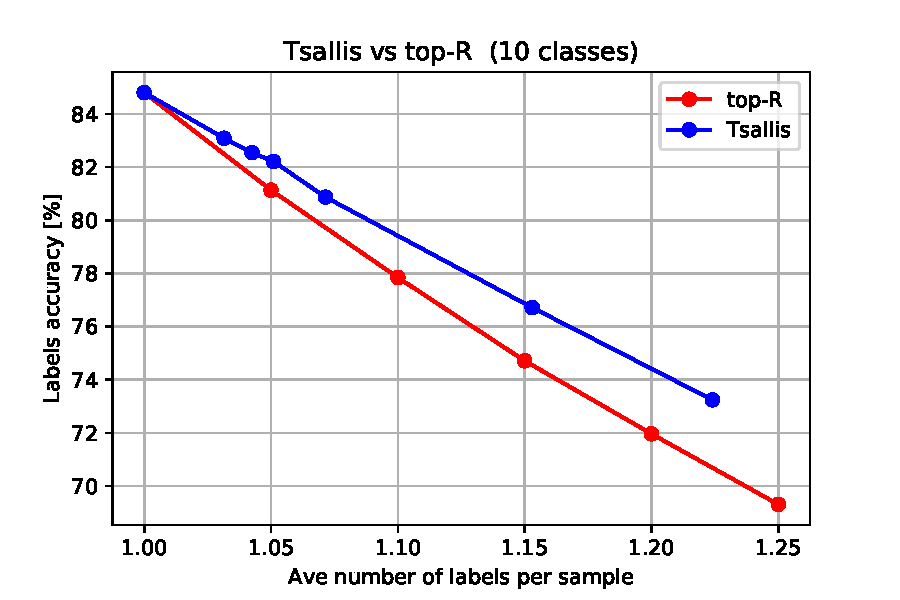
\includegraphics[width=1.0\linewidth]{figs/graphs/tsallis-vs-top-R-10cls.pdf}
    \caption{Tsallis entropy based labelling vs top-$r$ labelling (10 classes)}
    \label{fig:exp_10cls}
\end{center}
\end{figure}

実験結果を図~\ref{fig:exp_10cls}など(これは10クラスのものだが,他にどれを使うか?)に示す.ここでは横軸に平均ラベル数,縦軸にラベルの精度をとる.
全ての$K$クラス問題($2\leq K \leq 10$)において,同じ平均ラベル数でもTsallis entropy based labellingの精度がtop-$r$に勝ることが確認された.したがって,結果として同じ平均ラベル数のデータになるならば,どのインスタンスにいくつラベルを付与するかは,アノテータの自由意志に基づいて選択するほうが高精度なデータが得られるということが実験的に証明された.

\section{結論}
\begin{itemize}
    \item Tsallis entropy based labellingを提案した
    \item 理論的にどういうものなのか紹介した
    \item 他の一般的に考えられるモデルを包含することも示した
    \item MNISTでの実験で挙動を確認した
    \item 複数ラベルつけるデータを指定するよりも,自由に選ばせた方が同じ平均ラベル数でも精度が向上することを実験的に示した
\end{itemize}

% conference papers do not normally have an appendix

\section*{Acknowledgment}
%The authors would like to thank...

\bibliographystyle{IEEEtran}
\bibliography{IEEEabrv,mybib}

% that's all folks
\end{document}